% From Scratch to Python: a Google Colab workbook for a 9-year-old.
% Compile with:  tectonic scratch-to-python-workbook.tex
\documentclass[12pt,a4paper]{article}
\usepackage[a4paper,margin=2cm,top=2cm,bottom=2.2cm]{geometry}
\usepackage{fontspec}
\usepackage{FiraSans}
\setmonofont{FiraMono}[Extension=.otf, UprightFont=*-Regular, BoldFont=*-Bold, Ligatures=NoCommon]
\renewcommand{\familydefault}{\sfdefault}
\usepackage{xcolor}
\usepackage{amssymb}
\usepackage{array,longtable,booktabs}
\usepackage{enumitem}
\usepackage{needspace}
\newcolumntype{P}[1]{>{\raggedright\arraybackslash}p{#1}}
\usepackage{listings}
\usepackage[most]{tcolorbox}
\usepackage{tikz}
\usetikzlibrary{arrows.meta,calc,shapes.geometric}
\usepackage{scratch3}
\usepackage{fancyhdr}
\usepackage[hidelinks]{hyperref}

\linespread{1.22}
\setlength{\emergencystretch}{3em}
\setlength{\parindent}{0pt}
\setlength{\parskip}{7pt}
\setlist{itemsep=3pt,topsep=4pt}
\setscratch{scale=1, else word=else}

% ---------- Scratch colours ----------
\definecolor{motion}{HTML}{4C97FF}
\definecolor{looks}{HTML}{9966FF}
\definecolor{sound}{HTML}{CF63CF}
\definecolor{events}{HTML}{FFBF00}
\definecolor{control}{HTML}{FFAB19}
\definecolor{sensing}{HTML}{5CB1D6}
\definecolor{operators}{HTML}{59C059}
\definecolor{variables}{HTML}{FF8C1A}
\definecolor{lists}{HTML}{FF661A}
\definecolor{myblocks}{HTML}{FF6680}
\definecolor{pen}{HTML}{0FBD8C}
\definecolor{ink}{HTML}{1B2550}
\definecolor{muted}{HTML}{56618A}
\definecolor{codebg}{HTML}{F3F6FD}
\definecolor{codeframe}{HTML}{9AA8D4}
\definecolor{kw}{HTML}{1D4FC4}
\definecolor{str}{HTML}{1B7F3B}
\definecolor{com}{HTML}{7A84A8}
\definecolor{warnbg}{HTML}{FFF3DB}
\definecolor{warnframe}{HTML}{E89A12}
\definecolor{chalbg}{HTML}{E6F7EC}
\definecolor{chalframe}{HTML}{2E9C57}
\definecolor{thinkbg}{HTML}{E8F0FF}
\definecolor{thinkframe}{HTML}{4C7FE0}
\definecolor{errbg}{HTML}{FFECEC}
\definecolor{errframe}{HTML}{D23B3B}\colorlet{errhead}{errframe!35}
\color{ink}

% ---------- Python code ----------
\lstdefinestyle{py}{
  language=Python, basicstyle=\ttfamily\normalsize, keepspaces=true, columns=fixed,
  upquote=true, showstringspaces=false, keywordstyle=\color{kw}\bfseries,
  stringstyle=\color{str}, commentstyle=\color{com}\itshape,
  morekeywords={True,False,None}, deletekeywords={print,input,range,int,str,len,abs,round},
  numbers=left, numberstyle=\scriptsize\color{muted}, numbersep=9pt, xleftmargin=0pt,
  tabsize=4, breaklines=true
}
\lstdefinestyle{inl}{style=py, numbers=none, basicstyle=\ttfamily}
\newcommand{\py}{\lstinline[style=inl]}
\DeclareTextCommand{\textvisiblespace}{TU}{\makebox[0.6em][c]{\color{muted}\rule{0.5pt}{0.35ex}\rule{0.45em}{0.5pt}\rule{0.5pt}{0.35ex}}}
\makeatletter\def\lst@visiblespace{\textvisiblespace}\makeatother

\newtcblisting{typethis}[1][Type this into a code cell]{
  listing only, enhanced, colback=codebg, colframe=codeframe, boxrule=0.8pt, arc=6pt,
  left=22pt, right=8pt, top=4pt, bottom=4pt,
  title={\textbf{#1}}, coltitle=white, colbacktitle=ink, fonttitle=\small,
  listing options={style=py}}
\newtcblisting{code}{
  listing only, enhanced, colback=codebg, colframe=codeframe, boxrule=0.6pt, arc=5pt,
  left=22pt, right=6pt, top=2pt, bottom=2pt, listing options={style=py}}
\newtcblisting{codenonum}{
  listing only, enhanced, colback=codebg, colframe=codeframe, boxrule=0.6pt, arc=5pt,
  left=8pt, right=6pt, top=2pt, bottom=2pt, listing options={style=py,numbers=none}}
\newtcblisting{spaces}{
  listing only, enhanced, colback=codebg, colframe=codeframe, boxrule=0.6pt, arc=5pt,
  left=22pt, right=6pt, top=2pt, bottom=2pt, listing options={style=py,showspaces=true}}
\newtcolorbox{outputbox}[1][You should see]{
  enhanced, colback=white, colframe=ink!40, boxrule=0.6pt, arc=5pt, left=8pt,
  title={\textbf{#1}}, coltitle=ink, colbacktitle=ink!10, fonttitle=\small,
  fontupper=\ttfamily}

% ---------- Helper boxes ----------
\newtcolorbox{watchout}[1][Watch out!]{enhanced, breakable, colback=warnbg, colframe=warnframe,
  boxrule=0.8pt, arc=6pt, title={\textbf{#1}}, coltitle=ink, colbacktitle=warnframe!35, left=8pt, right=8pt}
\newtcolorbox{challenge}[1][Make it yours]{enhanced, breakable, colback=chalbg, colframe=chalframe,
  boxrule=0.8pt, arc=6pt, title={\textbf{#1}}, coltitle=white, colbacktitle=chalframe, left=8pt, right=8pt}
\newtcolorbox{think}[1][Did you notice?]{enhanced, breakable, colback=thinkbg, colframe=thinkframe,
  boxrule=0.8pt, arc=6pt, title={\textbf{#1}}, coltitle=white, colbacktitle=thinkframe, left=8pt, right=8pt}
\newtcolorbox{errorbox}{enhanced, colback=errbg, colframe=errframe, boxrule=0.8pt, arc=5pt,
  fontupper=\ttfamily\small, left=8pt}
\newtcbox{\chip}[1][motion]{on line, colback=#1!45!white, colframe=#1!80!black, boxrule=0.5pt,
  arc=7pt, left=4pt, right=4pt, top=0.5pt, bottom=0.5pt, boxsep=0pt, fontupper=\sffamily\small\bfseries}
\newcommand{\tick}{$\square$\ }
\newcommand{\step}[1]{\par\needspace{9\baselineskip}\medskip{\large\bfseries\color{ink}#1}\par}

% Colab "play" button drawn inline
\newcommand{\playbtn}{\tikz[baseline=-0.6ex]{\fill[ink] (0,0) circle (1.7ex); \fill[white] (-0.5ex,-0.8ex) -- (-0.5ex,0.8ex) -- (0.8ex,0) -- cycle;}}
\newcommand{\stopbtn}{\tikz[baseline=-0.6ex]{\draw[ink,line width=0.9pt] (0,0) circle (1.7ex); \fill[ink] (-0.6ex,-0.6ex) rectangle (0.6ex,0.6ex);}}

% Section banners
\newcommand{\banner}[3]{% colour, small label, title
  \clearpage
  \begin{tcolorbox}[enhanced, colback=#1, colframe=#1!80!black, arc=10pt, boxrule=0pt,
    left=14pt, top=10pt, bottom=10pt]
    {\small\bfseries\color{ink}#2}\par\vspace{2pt}
    {\fontsize{26}{30}\selectfont\bfseries\color{ink}#3}
  \end{tcolorbox}
  \addcontentsline{toc}{section}{#3}
  \vspace{4pt}}
\newcommand{\missionhead}[3]{% number, title, you will learn
  \clearpage
  \begin{tcolorbox}[enhanced, colback=ink, colframe=ink, arc=10pt, left=14pt, top=10pt, bottom=10pt]
    {\small\bfseries\color{events}MISSION #1}\par\vspace{2pt}
    {\fontsize{26}{30}\selectfont\bfseries\color{white}#2}\par\vspace{4pt}
    {\color{white}\textbf{You will learn:} #3}
  \end{tcolorbox}
  \addcontentsline{toc}{section}{Mission #1: #2}
  \vspace{2pt}}

\pagestyle{fancy}
\fancyhf{}
\renewcommand{\headrulewidth}{0pt}
\fancyfoot[C]{\small\color{muted}\thepage}
\fancyfoot[R]{\small\color{muted}From Scratch to Python}

\begin{document}

% =====================================================================
% COVER
% =====================================================================
\thispagestyle{empty}
\begin{tikzpicture}[remember picture, overlay]
  \fill[codebg] (current page.north west) rectangle (current page.south east);
  % a turtle-drawn star
  \begin{scope}[shift={($(current page.center)+(0,-1.2)$)}, line width=3pt, line join=round]
    \draw[looks] (-3.2,0.6) -- ++(0:6.4) -- ++(-144:6.4) -- ++(72:6.4) -- ++(-72:6.4) -- cycle;
  \end{scope}
  \foreach \c/\x in {motion/0, looks/1, events/2, control/3, operators/4, variables/5, myblocks/6, pen/7}
    \fill[\c] ($(current page.south west)+(\x*2.625,0)$) rectangle ++(2.625,1.1);
\end{tikzpicture}

\vspace*{1.2cm}
{\color{muted}\Large\bfseries A workbook for young coders}\par\vspace{6pt}
{\fontsize{46}{52}\selectfont\bfseries From Scratch\\[2pt] to Python}\par\vspace{10pt}
{\Large Using Google Colab}\par
\vspace{11.5cm}
\begin{tcolorbox}[colback=white, colframe=ink, arc=8pt, width=11cm, boxrule=1pt]
\Large This book belongs to:\par\vspace{9mm}\rule{9.5cm}{0.6pt}\par\vspace{2mm}
\end{tcolorbox}

% =====================================================================
\banner{events}{START HERE}{Hello, coder!}

You already know how to code. Every time you snap Scratch blocks together, you are writing a program. You tell the computer what to do, step by step.

In this book you will learn \textbf{Python}. Python is a real programming language. Grown-up programmers use it to build websites, games, robots and even space missions. The great news is that Python uses the \textbf{same ideas} as Scratch:

\begin{itemize}
  \item a \chip[motion]{move 100 steps} block becomes \py|t.forward(100)|
  \item a \chip[control]{repeat 4} block becomes \py|for i in range(4):|
  \item a \chip[looks]{say Hello!} block becomes \py|print("Hello!")|
\end{itemize}

The difference is that in Python you \textbf{type} the words instead of dragging blocks. That is the only big new thing. Everything else, like loops, variables and making your own blocks, you already understand.

\subsection*{How to use this book}

Go through the book in order. Each \textbf{mission} has five steps:

\begin{enumerate}[label=\textbf{\arabic*.}]
  \item \textbf{Build it in Scratch.} Make the program in Scratch first, so you know what it should do.
  \item \textbf{Type it in Colab.} Copy the Python code into Colab, letter by letter.
  \item \textbf{Read it line by line.} Find out which Scratch block each line matches.
  \item \textbf{Run it.} Press the play button and check that it worked.
  \item \textbf{Make it yours.} Change the program and see what happens.
\end{enumerate}

\needspace{16\baselineskip}
Look out for these boxes:

\begin{tcbraster}[raster columns=2, raster equal height, raster column skip=8pt]
\begin{typethis}[Type this]
print("Hi!")
\end{typethis}
\begin{watchout}
A mistake lots of people make, so you can avoid it.
\end{watchout}
\begin{think}
Something clever to spot in the code.
\end{think}
\begin{challenge}
Ideas for changing the program. Tick each one you finish!
\end{challenge}
\end{tcbraster}

\subsection*{My missions}
Colour in a star each time you finish a mission.

\begin{center}
\begin{tabular}{lll}
\toprule
\textbf{Mission} & \textbf{What you make} & \textbf{Done?} \\
\midrule
1 & Say hello & $\star$\ \ $\star$\ \ $\star$ \\
2 & Draw shapes & $\star$\ \ $\star$\ \ $\star$ \\
3 & Guess my number & $\star$\ \ $\star$\ \ $\star$ \\
4 & Make your own block & $\star$\ \ $\star$\ \ $\star$ \\
5 & Turtle race & $\star$\ \ $\star$\ \ $\star$ \\
Bonus & Translate it yourself & $\star$\ \ $\star$\ \ $\star$ \\
\bottomrule
\end{tabular}
\end{center}
One star for making it work, two for doing one challenge, and three for doing them all!

% =====================================================================
\banner{sensing}{GETTING READY}{Meet Google Colab}

\textbf{Google Colab} is a website where you can write Python and run it straight away. You don't have to install anything. Colab saves your work in Google Drive, so it will be there next time.

\step{Step 1: Open Colab}
Ask a grown-up to open this website and sign in with a Google account:
\begin{center}\Large\texttt{colab.research.google.com}\end{center}

\step{Step 2: Make a new notebook}
Click \textbf{New notebook}. A notebook is like a Scratch project: it is where your code lives.

At the top it says \texttt{Untitled0.ipynb}. Click on that name and change it to \textbf{My Python Adventures}.

\step{Step 3: Find the code cell}
You will see a grey box with a round button on the left. This box is called a \textbf{code cell}. You type Python into it.

\begin{center}
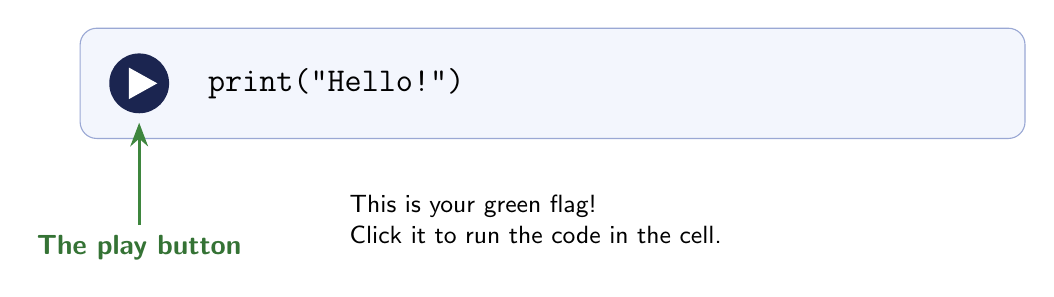
\begin{tikzpicture}
  \draw[codeframe, fill=codebg, rounded corners=6pt] (0,0) rectangle (12,1.4);
  \fill[ink] (0.75,0.7) circle (0.38);
  \fill[white] (0.62,0.5) -- (0.62,0.9) -- (0.98,0.7) -- cycle;
  \node[anchor=west, font=\ttfamily\large] at (1.5,0.7) {print("Hello!")};
  \draw[-{Stealth[length=3mm]}, line width=1.2pt, operators!70!black] (0.75,-1.1) -- (0.75,0.2);
  \node[anchor=north, font=\bfseries, text=operators!60!black] at (0.75,-1.1) {The play button};
  \node[anchor=north west, align=left, font=\small] at (3.3,-0.6) {This is your green flag!\\ Click it to run the code in the cell.};
\end{tikzpicture}
\end{center}

\step{Step 4: Say hello}
Click inside the cell and type this exactly:

\begin{typethis}
print("Hello!")
\end{typethis}

Now click the play button \playbtn. You can also hold \textbf{Shift} and press \textbf{Enter}. The first time, it may take a few seconds to start. Then you will see this underneath:

\begin{outputbox}
Hello!
\end{outputbox}

\textbf{You just ran your first Python program!}

\step{Step 5: Add more cells}
Click \textbf{+ Code} at the top to get a new empty cell. Use a new cell for each program. You can run any cell again whenever you like.

\needspace{14\baselineskip}
\subsection*{The magic first cell: getting the turtle}

In Scratch, you get pen blocks by clicking the \textbf{Extensions} button in the bottom corner. Python works the same way. We add the drawing tools that we need, which in Python are called a \textbf{turtle}.

In Python, the sprite is a \textbf{turtle} that walks around and draws lines. It is just like Scratch with the \chip[pen]{pen down} block.

Each time you open your notebook, run this cell first:

\begin{typethis}[Magic first cell: run it once every time you open Colab]
!pip install ColabTurtlePlus
\end{typethis}

The \texttt{!} at the start means: ``this isn't Python. It is an instruction for Colab to download the turtle tools.'' Lots of text will scroll past. That is fine. Wait until it stops.

\needspace{18\baselineskip}
\subsection*{The four starting lines}

Every program that draws starts with these four lines. They do the same job as this Scratch block:\par\chip[events]{when green flag clicked}

\begin{typethis}[Start every drawing with these lines]
from ColabTurtlePlus.Turtle import *
clearscreen()
setup(480, 360)
t = Turtle()
\end{typethis}

\begin{longtable}{>{\centering\arraybackslash}p{0.8cm} P{14.5cm}}
\toprule
\textbf{Line} & \textbf{What it does} \\
\midrule
1 & \textbf{Bring in the turtle tools.} This is like clicking Extensions and choosing Pen. \\
2 & \textbf{Clear the stage.} It wipes away the old drawing so you can start fresh. \\
3 & \textbf{Make the stage 480 wide and 360 tall.} That is exactly the same size as the Scratch stage! \\
4 & \textbf{Make a sprite called} \texttt{t}. From now on, \py|t.| means ``hey turtle, do this''. So \py|t.forward(100)| means ``turtle, move 100 steps''. \\
\bottomrule
\end{longtable}

When you run them, Colab may show a message about \py|clearscreen()|. That is just a reminder, and you can ignore it.

\begin{watchout}[If Colab gets stuck or forgets]
\begin{itemize}
  \item \textbf{A cell keeps running forever?} Click the \stopbtn{} button where the play button was. This is just like the red stop sign in Scratch.
  \item \textbf{You see \texttt{No module named 'ColabTurtlePlus'}?} Colab forgets everything when you close it or leave it alone for a while. Run the magic first cell again.
  \item \textbf{You see a \texttt{NameError}?} Run the cells above it first, starting from the top.
\end{itemize}
\end{watchout}

% =====================================================================
\banner{motion}{THE BIG PICTURE}{Scratch words, Python words}

Here are the Scratch things you know, and what Python calls them.

\begin{center}
\renewcommand{\arraystretch}{1.35}
\begin{tabular}{P{5.3cm} P{5.6cm} P{4.6cm}}
\toprule
\textbf{In Scratch} & \textbf{In Python with Colab} & \textbf{Example} \\
\midrule
A sprite & A turtle & \py|t = Turtle()| \\
The stage & The drawing area & \py|setup(480, 360)| \\
The green flag & The play button \playbtn & \\
The stop sign & The stop button \stopbtn & \\
A block & A line of code & \py|t.forward(10)| \\
Extensions button & \texttt{import} & \py|import random| \\
A white input bubble & Brackets \texttt{( )} & \py|t.right(90)| \\
Words in a bubble & Words in quote marks & \py|"Hello!"| \\
Make a Variable & Just give it a value & \py|score = 0| \\
My Blocks & A function & \py|def jump():| \\
\bottomrule
\end{tabular}
\end{center}

\subsection*{The stage is the same}

Good news: the turtle's stage has the same coordinates as the Scratch stage. The middle is $(0,0)$. $x$ goes from $-240$ on the left to $240$ on the right. $y$ goes from $-180$ at the bottom to $180$ at the top.

\begin{center}
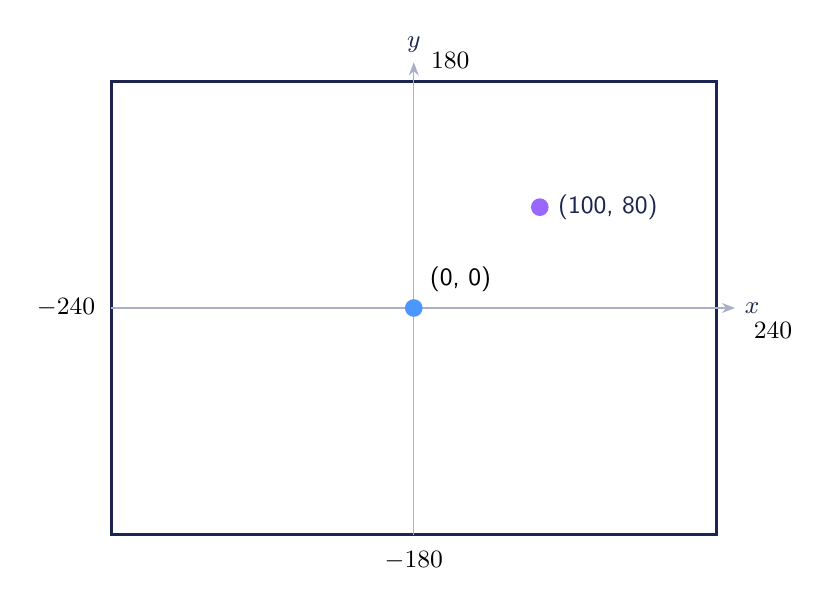
\begin{tikzpicture}[scale=0.016]
  \draw[ink, line width=1pt, fill=white] (-240,-180) rectangle (240,180);
  \draw[muted!50, -{Stealth}] (-240,0) -- (255,0) node[right, font=\small, text=ink] {$x$};
  \draw[muted!50, -{Stealth}] (0,-180) -- (0,195) node[above, font=\small, text=ink] {$y$};
  \fill[motion] (0,0) circle (7);
  \node[font=\small, anchor=south west] at (5,5) {(0, 0)};
  \node[font=\small, anchor=east] at (-245,0) {$-240$};
  \node[font=\small, anchor=west] at (262,-18) {$240$};
  \node[font=\small, anchor=north] at (0,-185) {$-180$};
  \node[font=\small, anchor=south west] at (6,182) {$180$};
  \fill[looks] (100,80) circle (7) node[right, font=\small, text=ink] {\ (100, 80)};
\end{tikzpicture}
\end{center}

\subsection*{But the directions are different!}

\begin{watchout}[Watch out: the compass is turned]
In Scratch, \chip[motion]{point in direction 90} points to the \textbf{right}, and 0 points \textbf{up}.

In Python, \py|t.setheading(0)| points to the \textbf{right}, and 90 points \textbf{up}.
\end{watchout}

\begin{center}
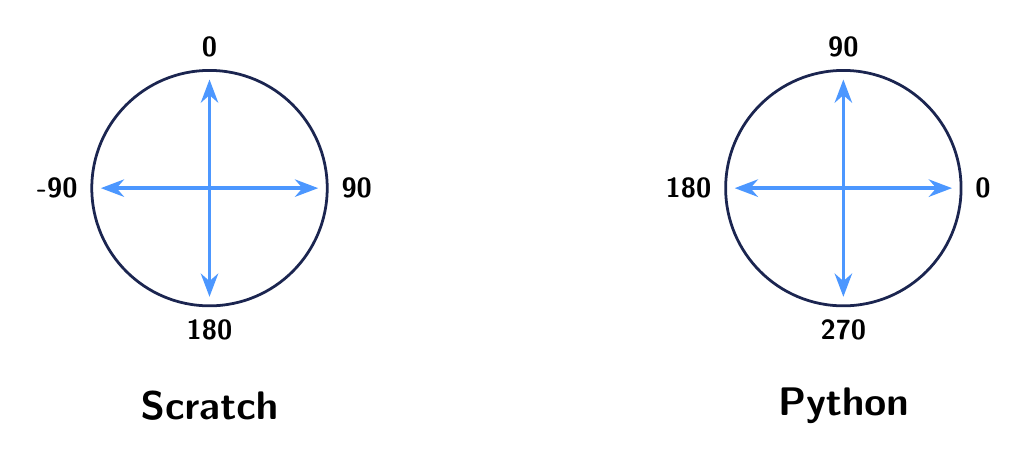
\begin{tikzpicture}[scale=1.15]
  \foreach \cx/\title/\up/\right/\down/\left in {0/Scratch/0/90/180/-90, 7/Python/90/0/270/180}{
    \begin{scope}[shift={(\cx,0)}]
      \draw[ink, line width=1pt] (0,0) circle (1.3);
      \draw[-{Stealth}, line width=1.2pt, motion] (0,0) -- (0,1.2);
      \draw[-{Stealth}, line width=1.2pt, motion] (0,0) -- (1.2,0);
      \draw[-{Stealth}, line width=1.2pt, motion] (0,0) -- (0,-1.2);
      \draw[-{Stealth}, line width=1.2pt, motion] (0,0) -- (-1.2,0);
      \node[above, font=\bfseries] at (0,1.35) {\up};
      \node[right, font=\bfseries] at (1.35,0) {\right};
      \node[below, font=\bfseries] at (0,-1.35) {\down};
      \node[left, font=\bfseries] at (-1.35,0) {\left};
      \node[font=\Large\bfseries] at (0,-2.4) {\title};
    \end{scope}}
\end{tikzpicture}
\end{center}

\begin{think}[The secret rule]
To turn any Scratch direction into a Python direction, take it away from 90:
\begin{center}\textbf{Python direction} $=$ \textbf{90} $-$ \textbf{Scratch direction}\end{center}
So \chip[motion]{point in direction 180} (down) is \py|t.setheading(90 - 180)|, which is $-90$. Python understands $-90$ too!
\end{think}

The good news is that \textbf{turning} works the same. \chip[motion]{turn right 90 degrees} is \py|t.right(90)|, and \chip[motion]{turn left 90 degrees} is \py|t.left(90)|. Most of the time you will use turning, not directions.

% =====================================================================
\banner{control}{THE BIG PICTURE}{Four new habits}

Python understands the same ideas as Scratch. But because you type instead of snapping blocks, there are four new habits to learn.

\subsection*{Habit 1: Spaces show what is inside}

In Scratch, a block goes \textbf{inside} a loop when you drop it into the C-shaped mouth.

In Python, two things do that job:
\begin{enumerate}
  \item a \textbf{colon} \texttt{:} at the end of the line opens the mouth.
  \item \textbf{four spaces} at the start of a line put it inside.
\end{enumerate}

\begin{tcbraster}[raster columns=2, raster equal height=rows, raster column skip=12pt, raster valign=center]
\begin{tcolorbox}[colback=white, colframe=white, boxrule=0pt, valign=center]
\begin{scratch}
\blockrepeat{repeat \ovalnum{4}}{
  \blockmove{move \ovalnum{100} steps}
  \blockmove{turn \turnright{} \ovalnum{90} degrees}
}
\blockpen{pen up}
\end{scratch}
\end{tcolorbox}
\begin{spaces}
for i in range(4):
    t.forward(100)
    t.right(90)
t.penup()
\end{spaces}
\end{tcbraster}

The little \texttt{\textvisiblespace} marks show the spaces, which are normally invisible. Lines 2 and 3 have four spaces, so they are \textbf{inside} the loop and repeat 4 times. Line 4 has no spaces, so it is \textbf{outside} the loop. It happens once, after the loop has finished.

\begin{think}[Colab helps you]
When you type a colon \texttt{:} and press Enter, Colab adds the four spaces for you. To come back out of the loop, press \textbf{Backspace} once.
\end{think}

\subsection*{Habit 2: Spell it exactly}

Blocks are already spelled for you. In Python, you do the spelling, and Python is very fussy. Capital letters, dots, brackets and quote marks must all be just right.

\begin{center}
\renewcommand{\arraystretch}{1.3}
\begin{tabular}{P{4.6cm} P{10.5cm}}
\toprule
\py|t.forward(100)| & \textbf{Works!} \\
\py|t.Forward(100)| & \textbf{Error:} capital F. Python thinks \texttt{Forward} and \texttt{forward} are different words. \\
\py|t.foward(100)| & \textbf{Error:} missing r. Python can't guess what you meant. \\
\py|t.forward 100| & \textbf{Error:} no brackets around 100. \\
\py|print("Hi)| & \textbf{Error:} the closing quote mark is missing. \\
\bottomrule
\end{tabular}
\end{center}

\begin{think}[Rule of pairs]
Brackets and quotes always come in pairs, just like socks! Every \texttt{(} needs a \texttt{)}, and every \texttt{"} needs another \texttt{"}.
\end{think}

\needspace{14\baselineskip}
\subsection*{Habit 3: One line at a time, from the top}

In Scratch, you can have lots of scripts that all start when you click the green flag. They all run at the same time.

Python is different. It reads your cell like a book: line 1, then line 2, then line 3, all the way to the bottom. It only jumps around when a loop or one of your own functions tells it to.

\begin{tcbraster}[raster columns=2, raster equal height=rows, raster column skip=12pt, raster valign=center]
\begin{tcolorbox}[colback=white, colframe=white, boxrule=0pt, valign=center]
\begin{scratch}
\blockinit{when \greenflag clicked}
\blocklook{say \ovalnum{first}}
\blocklook{say \ovalnum{second}}
\blocklook{say \ovalnum{third}}
\end{scratch}
\end{tcolorbox}
\begin{code}
print("first")
print("second")
print("third")
\end{code}
\end{tcbraster}

\needspace{24\baselineskip}
\subsection*{Habit 4: One = sets, two == checks}

Scratch has two different blocks: one to \textbf{set} a variable and one to \textbf{check} whether it equals something. Python uses equals signs for both, so it needs a way to tell them apart:

\begin{itemize}
  \item \textbf{One} equals sign \texttt{=} means ``put this value in the box''. It is like \chip[variables]{set score to 0}.
  \item \textbf{Two} equals signs \texttt{==} mean ``are these the same?''. It is like the green \chip[operators]{\ = \ } block.
\end{itemize}

\begin{tcbraster}[raster columns=2, raster equal height=rows, raster column skip=12pt, raster valign=center]
\begin{tcolorbox}[colback=white, colframe=white, boxrule=0pt, valign=center]
\begin{scratch}
\blockvariable{set \selectmenu{score} to \ovalnum{5}}
\blockif{if \booloperator{\ovalvariable{score} = \ovalnum{5}} then}{
  \blocklook{say \ovalnum{You win!}}
}
\end{scratch}
\end{tcolorbox}
\begin{code}
score = 5
if score == 5:
    print("You win!")
\end{code}
\end{tcbraster}

% =====================================================================
\missionhead{1}{Say hello}{\texttt{print}, \texttt{input}, variables and joining words with \texttt{+}}

In this mission, the computer asks your name and then says hello to you.

\step{Step 1: Build it in Scratch}

\begin{center}
\begin{scratch}
\blockinit{when \greenflag clicked}
\blocksensing{ask \ovalnum{What's your name?} and wait}
\blocklook{say \ovaloperator{join \ovalnum{Hello } \ovalsensing{answer}}}
\end{scratch}
\end{center}

\step{Step 2: Type it in Colab}
Make a new cell with \textbf{+ Code}. This one doesn't draw, so you don't need the turtle lines.

\begin{typethis}
answer = input("What's your name? ")
print("Hello " + answer)
\end{typethis}

\step{Step 3: Read it line by line}

\begin{longtable}{>{\centering\arraybackslash}p{1.1cm} P{6.1cm} P{8.3cm}}
\toprule
\textbf{Line} & \textbf{Scratch block} & \textbf{What it means} \\
\midrule
--- & \chip[events]{when green flag clicked} & No code needed. The play button \playbtn{} starts it. \\
1 & \chip[sensing]{ask What's your name? and wait} & \py|input(...)| asks the question and waits for you to type. Your answer goes into a variable called \py|answer|. \\
2 & \chip[looks]{say join Hello answer} & \py|print(...)| shows words below the cell. The \texttt{+} sign joins two pieces of writing together, just like the \chip[operators]{join} block. \\
\bottomrule
\end{longtable}

\step{Step 4: Run it}
Press \playbtn. A box appears under the cell. Type your name in it and press \textbf{Enter}.

\begin{outputbox}
What's your name? Ada\\
Hello Ada
\end{outputbox}

\begin{think}
Look at the space after \texttt{Hello} in \py|"Hello "|. Try taking it out and running it again. You will get \texttt{HelloAda}! Computers do \textbf{exactly} what you say, even with spaces.
\end{think}

\begin{watchout}[Watch out: words need quote marks]
\py|"Hello "| has quote marks, so Python knows it is writing to show on screen. \py|answer| has no quote marks, so Python knows it is the name of a variable. If you type \py|print("answer")|, Python will show the word \texttt{answer}, not your name!
\end{watchout}

\begin{challenge}
\tick Ask a second question, \py|food = input("What's your favourite food? ")|, then print a sentence with both answers, like \texttt{Ada loves pizza}.\par
\tick Make the computer say three different things, one after another. You need three \py|print| lines.\par
\tick \textbf{Super challenge:} ask for a number and print it 3 times using \py|print(answer * 3)|. What happens? (It's a bit of a surprise!)
\end{challenge}

% =====================================================================
\missionhead{2}{Draw shapes}{the turtle, \texttt{for} loops, pen colour and size}

Now let's draw! The turtle walks around the stage with its pen down and leaves a line behind it.

\step{Step 1: Build it in Scratch}
Click Extensions and add \textbf{Pen}, then build:

\begin{center}
\begin{scratch}
\blockinit{when \greenflag clicked}
\blockpen{pen down}
\blockpen{set pen color to \ovalnum{blue}}
\blockpen{set pen size to \ovalnum{3}}
\blockrepeat{repeat \ovalnum{4}}{
  \blockmove{move \ovalnum{100} steps}
  \blockmove{turn \turnright{} \ovalnum{90} degrees}
}
\end{scratch}
\end{center}

\step{Step 2: Type it in Colab}

\begin{typethis}
from ColabTurtlePlus.Turtle import *
clearscreen()
setup(480, 360)
t = Turtle()
t.pencolor("blue")
t.pensize(3)
for i in range(4):
    t.forward(100)
    t.right(90)
\end{typethis}

\step{Step 3: Read it line by line}

\begin{longtable}{>{\centering\arraybackslash}p{1.1cm} P{5.3cm} P{9.1cm}}
\toprule
\textbf{Line} & \textbf{Scratch block} & \textbf{What it means} \\
\midrule
1--4 & \chip[events]{when green flag clicked} & The four starting lines. They get the stage and the turtle ready. The turtle's pen starts \textbf{down}, so you don't need \chip[pen]{pen down}. \\
5 & \chip[pen]{set pen color to blue} & Colours are words in quote marks, like \py|"red"|, \py|"gold"| or \py|"purple"|. \\
6 & \chip[pen]{set pen size to 3} & A bigger number draws a thicker line. \\
7 & \chip[control]{repeat 4} & \py|for i in range(4):| means ``do this 4 times''. Don't forget the colon! \\
8 & \chip[motion]{move 100 steps} & It has four spaces in front, so it is inside the loop. \\
9 & \chip[motion]{turn right 90 degrees} & This is inside the loop too. \\
\bottomrule
\end{longtable}

\step{Step 4: Run it}
Press \playbtn. You should see the turtle draw a blue square.

\begin{think}[What is the i for?]
The \texttt{i} counts how many times the loop has gone round. Python starts counting at \textbf{0}, so \texttt{i} is 0, then 1, then 2, then 3. That's still 4 times! You don't have to use \texttt{i}, but it is there if you want it.
\end{think}

\needspace{14\baselineskip}
\step{Step 5: Make it yours}

Here is a trick: \textbf{the turns in any shape add up to 360 degrees}. To work out the turn, divide 360 by the number of sides. Fill in the table, then draw each shape by changing the numbers in lines 7 and 9.

\begin{center}
\renewcommand{\arraystretch}{1.5}
\begin{tabular}{P{3.6cm} P{3.4cm} P{3.4cm} P{1.6cm}}
\toprule
\textbf{Shape} & \textbf{Sides (repeat)} & \textbf{Turn} & \textbf{Drawn?} \\
\midrule
Triangle & 3 & $360 \div 3 = 120$ & $\square$ \\
Square & 4 & $360 \div 4 = 90$ & $\square$ \\
Pentagon & 5 & \rule{2.2cm}{0.5pt} & $\square$ \\
Hexagon & 6 & \rule{2.2cm}{0.5pt} & $\square$ \\
Octagon & 8 & \rule{2.2cm}{0.5pt} & $\square$ \\
\bottomrule
\end{tabular}
\end{center}

\begin{challenge}
\tick \textbf{Draw a star.} Use \texttt{5} for the repeat, \texttt{150} for the move, and turn \texttt{144}. (A star turns twice as far as a pentagon!)\par
\tick Change the pen colour to your favourite colour.\par
\tick Put \py|t.pencolor("red")| \textbf{inside} the loop, before the forward line. Does anything change? Now try changing the colour \textbf{half way round}.\par
\tick Make the turtle look like a turtle with \py|t.shape("turtle")|, and draw faster with \py|t.speed(13)|. Add both lines just after line 4.
\end{challenge}

\begin{watchout}
If the turtle draws one long line instead of a shape, check your spaces. The turn line must have four spaces in front, just like the forward line, so that it is inside the loop too.
\end{watchout}

% =====================================================================
\missionhead{3}{Guess my number}{\texttt{random}, \texttt{while} loops, \texttt{if} and turning words into numbers}

The computer picks a secret number from 1 to 10. You keep guessing until you get it right, and it tells you whether each guess is too low or too high.

\step{Step 1: Build it in Scratch}
Make two variables called \textbf{secret} and \textbf{guess}, then build:

\begin{center}
\begin{scratch}
\blockinit{when \greenflag clicked}
\blockvariable{set \selectmenu{secret} to \ovaloperator{pick random \ovalnum{1} to \ovalnum{10}}}
\blockvariable{set \selectmenu{guess} to \ovalnum{0}}
\blockrepeat{repeat until \booloperator{\ovalvariable{guess} = \ovalvariable{secret}}}{
  \blocksensing{ask \ovalnum{Guess 1 to 10:} and wait}
  \blockvariable{set \selectmenu{guess} to \ovalsensing{answer}}
  \blockif{if \booloperator{\ovalvariable{guess} < \ovalvariable{secret}} then}{
    \blocklook{say \ovalnum{Too low} for \ovalnum{1} seconds}
  }
  \blockif{if \booloperator{\ovalvariable{guess} > \ovalvariable{secret}} then}{
    \blocklook{say \ovalnum{Too high} for \ovalnum{1} seconds}
  }
}
\blocklook{say \ovalnum{You got it!}}
\end{scratch}
\end{center}

\step{Step 2: Type it in Colab}

\begin{typethis}
import random
secret = random.randint(1, 10)
guess = 0
while guess != secret:
    guess = int(input("Guess 1 to 10: "))
    if guess < secret:
        print("Too low")
    if guess > secret:
        print("Too high")
print("You got it!")
\end{typethis}

\needspace{14\baselineskip}
\step{Step 3: Read it line by line}

\begin{longtable}{>{\centering\arraybackslash}p{1.1cm} P{5.5cm} P{8.9cm}}
\toprule
\textbf{Line} & \textbf{Scratch block} & \textbf{What it means} \\
\midrule
1 & (Extensions) & Brings in Python's random number tools. \\
2 & \chip[variables]{set secret to pick random} & \py|random.randint(1, 10)| picks a whole number from 1 to 10. It can pick 1 or 10, just like Scratch. \\
3 & \chip[variables]{set guess to 0} & Makes the variable \py|guess| and puts 0 in it. \\
4 & \chip[control]{repeat until guess = secret} & \py|while guess != secret:| \texttt{!=} means ``is \textbf{not} equal to''. Look at the box below! \\
5 & \chip[sensing]{ask} and \chip[variables]{set guess to answer} & Two blocks in one line! It asks, turns your answer into a number with \py|int( )|, and stores it in \py|guess|. \\
6--7 & \chip[control]{if guess < secret then} & If the guess is smaller, say ``Too low''. \\
8--9 & \chip[control]{if guess > secret then} & If the guess is bigger, say ``Too high''. \\
10 & \chip[looks]{say You got it!} & It has no spaces in front, so it runs once the loop is finished. \\
\bottomrule
\end{longtable}

\begin{watchout}[Watch out: Python flips the question]
Scratch says \textbf{repeat until} the guess \textbf{equals} the secret.

Python says keep going \textbf{while} the guess does \textbf{not equal} the secret.

It means the same thing said the other way round, like ``stay outside until it rains'' and ``stay outside while it isn't raining''.
\end{watchout}

\begin{think}[Why do we need \texttt{int( )}?]
Whatever you type into \py|input| is \textbf{writing} to Python, even if it looks like a number. \texttt{"7"} in quote marks is writing. \texttt{7} without quote marks is a number. Python can't work out whether writing is smaller than a number, so \py|int( )| turns the writing into a real number first. (Scratch does this for you without telling you!)
\end{think}

\step{Step 4: Run it}
Press \playbtn{} and type guesses into the box. Press Enter after each one.

\begin{outputbox}[You might see]
Guess 1 to 10: 5\\
Too low\\
Guess 1 to 10: 8\\
Too high\\
Guess 1 to 10: 7\\
You got it!
\end{outputbox}

\begin{challenge}
\tick Make it harder: pick a number from 1 to \textbf{100}. Remember to change the question too!\par
\tick \textbf{Count your guesses.} Add \py|tries = 0| before the loop and \py|tries = tries + 1| inside it. At the end, print \py|"You took " + str(tries) + " tries"|. (Why do you think \py|str( )| is needed? Look at the Did you notice? box again.)\par
\tick Type \texttt{cat} as a guess. Python shows a red error. Read the last line of it. Can you work out what went wrong?
\end{challenge}

% =====================================================================
\missionhead{4}{Make your own block}{functions with \texttt{def}, and inputs}

In Scratch, \textbf{My Blocks} lets you make your own block, like \chip[myblocks]{square}. In Python this is called a \textbf{function}, and you make one with the word \py|def| (short for \emph{define}).

\step{Step 1: Build it in Scratch}
Click \textbf{My Blocks}, then \textbf{Make a Block}. Call it \texttt{square}, and add a number input called \texttt{size}.

\begin{center}
\begin{tabular}{c@{\hspace{1.2cm}}c}
\begin{scratch}
\initmoreblocks{define \namemoreblocks{square \ovalmoreblocks{size}}}
\blockrepeat{repeat \ovalnum{4}}{
  \blockmove{move \ovalmoreblocks{size} steps}
  \blockmove{turn \turnright{} \ovalnum{90} degrees}
}
\end{scratch}
&
\begin{scratch}
\blockinit{when \greenflag clicked}
\blockpen{pen down}
\blockmoreblocks{square \ovalnum{40}}
\blockmoreblocks{square \ovalnum{80}}
\blockmoreblocks{square \ovalnum{120}}
\end{scratch}
\end{tabular}
\end{center}

\step{Step 2: Type it in Colab}

\begin{typethis}
from ColabTurtlePlus.Turtle import *
clearscreen()
setup(480, 360)
t = Turtle()

def square(size):
    for i in range(4):
        t.forward(size)
        t.right(90)

square(40)
square(80)
square(120)
\end{typethis}

\step{Step 3: Read it line by line}

\begin{longtable}{>{\centering\arraybackslash}p{1.1cm} P{5.1cm} P{9.3cm}}
\toprule
\textbf{Line} & \textbf{Scratch block} & \textbf{What it means} \\
\midrule
1--4 & & The four starting lines. \\
6 & \chip[myblocks]{define square (size)} & \py|def square(size):| makes a new block called \py|square| with an input called \py|size|. The colon opens it up. \\
7--9 & \chip[control]{repeat 4} \ldots & These lines are indented, so they are \textbf{inside} the function. This is what \texttt{square} does. Lines 8 and 9 have \textbf{eight} spaces, because they are inside the loop, which is inside the function! \\
11 & \chip[myblocks]{square 40} & This \textbf{uses} your block. The 40 goes into \py|size|. \\
12--13 & \chip[myblocks]{square 80} \chip[myblocks]{square 120} & Use it again with bigger sizes. You wrote the square code once, but you used it three times! \\
\bottomrule
\end{longtable}

\step{Step 4: Run it}
You should see three squares of different sizes, all starting from the same corner.

\begin{watchout}[Watch out: define it first]
Python reads from the top, so the \py|def| part must be \textbf{above} the lines that use it. If \py|square(40)| comes before \py|def square|, Python says \texttt{NameError}, because it hasn't learned the word yet.
\end{watchout}

\begin{challenge}
\tick Make a \py|triangle(size)| function. It works like \texttt{square}, but repeats 3 times and turns 120.\par
\tick \textbf{Draw a flower.} Add this at the bottom and run it. (Add \py|t.speed(13)| after line 4 so it doesn't take ages.)
\begin{codenonum}
for i in range(12):
    square(80)
    t.right(30)
\end{codenonum}
\tick Give your function a second input for the colour: \py|def square(size, colour):|, then add \py|t.pencolor(colour)| as the first line inside. Use it like this: \py|square(80, "red")|.
\end{challenge}

% =====================================================================
\missionhead{5}{Turtle race}{two sprites, random numbers, \texttt{and}, and \texttt{if}/\texttt{else}}

Two turtles race across the stage. Each turn, they move forward by a random amount. Who will win? Even the computer doesn't know!

\step{Step 1: Build it in Scratch}
Make two sprites called \textbf{Red} and \textbf{Blue}. The red one gets this script, and the blue one gets the same script with $y = -50$:

\begin{center}
\begin{scratch}
\blockinit{when \greenflag clicked}
\blockpen{pen up}
\blockmove{go to x: \ovalnum{-200} y: \ovalnum{50}}
\blockpen{pen down}
\blockrepeat{repeat until \booloperator{\ovalmove{x position} > \ovalnum{200}}}{
  \blockmove{change x by \ovaloperator{pick random \ovalnum{1} to \ovalnum{20}}}
}
\blocklook{say \ovalnum{I win!}}
\end{scratch}
\end{center}

In Scratch, each sprite runs its own script \textbf{at the same time}. Python works one line at a time (Habit 3!), so in Python \textbf{one loop moves both turtles}, one step each, again and again.

\step{Step 2: Type it in Colab}

\begin{typethis}
from ColabTurtlePlus.Turtle import *
import random
clearscreen()
setup(480, 360)

red = Turtle()
red.shape("turtle")
red.color("red")
red.penup()
red.goto(-200, 50)
red.pendown()

blue = Turtle()
blue.shape("turtle")
blue.color("blue")
blue.penup()
blue.goto(-200, -50)
blue.pendown()

while red.xcor() < 200 and blue.xcor() < 200:
    red.forward(random.randint(1, 20))
    blue.forward(random.randint(1, 20))

if red.xcor() > blue.xcor():
    print("Red wins!")
else:
    print("Blue wins!")
\end{typethis}

\needspace{14\baselineskip}
\step{Step 3: Read it line by line}

\begin{longtable}{>{\centering\arraybackslash}p{1.1cm} P{5.2cm} P{9.2cm}}
\toprule
\textbf{Line} & \textbf{Scratch block} & \textbf{What it means} \\
\midrule
1--4 & & The starting lines, plus \py|import random|. \\
6 & (a new sprite) & \py|red = Turtle()| makes a sprite and calls it \texttt{red} instead of \texttt{t}. \\
7--8 & \chip[looks]{switch costume} & The turtle shape, coloured red. \\
9--11 & \chip[pen]{pen up}\newline\chip[motion]{go to x: -200 y: 50}\newline\chip[pen]{pen down} & Go to the start line without drawing, then put the pen down. \\
13--18 & & The same again for a second sprite called \texttt{blue}. \\
20 & \chip[control]{repeat until} \ldots & Keep going \textbf{while} red has not crossed 200 \textbf{and} blue has not crossed 200. \texttt{and} means both have to be true, like the green \chip[operators]{and} block. \\
21--22 & \chip[motion]{change x by pick random} & Each turtle walks forward by a random number of steps. \\
24--27 & \chip[control]{if then else} & If red is further right, red wins. \textbf{Otherwise} (that is what \py|else:| means) blue wins. \\
\bottomrule
\end{longtable}

\step{Step 4: Run it}
Watch the turtles race! Below the drawing, you will see \texttt{Red wins!} or \texttt{Blue wins!}. Run it again. Do you get the same winner every time?

\begin{think}[\texttt{red.} and \texttt{blue.}]
The word before the dot tells Python \textbf{which sprite} you are talking to. \py|red.forward(10)| moves only the red turtle. In Scratch, you choose a sprite by clicking on it. In Python, you write its name in front of the dot.
\end{think}

\begin{challenge}
\tick Add a third, \textbf{green} turtle at $y = 0$. You'll need to change lines 20, 21 and 24. (Hint: three turtles means \texttt{and} twice.)\par
\tick Make the race longer: start at $-230$ and finish at $230$.\par
\tick Make one turtle a cheater: let it move \py|random.randint(1, 25)|. Run the race 5 times. Who wins most?\par
\tick Draw a finish line before the race starts, using another turtle called \py|line| that goes to $(200, 150)$ and walks down to $(200, -150)$.
\end{challenge}

\begin{center}
\begin{tcolorbox}[colback=ink, colframe=ink, arc=10pt, width=13cm, halign=center]
{\color{white}\Large\bfseries Well done, Python coder!}\par\vspace{4pt}
{\color{white}You have finished all five missions. You can now write programs in two languages: blocks and Python!}
\end{tcolorbox}
\end{center}

% =====================================================================
\banner{pen}{YOUR TURN}{Translate it yourself}

Now you are the translator! Here are two Scratch scripts you haven't seen before. For each one:

\begin{enumerate}[label=\textbf{\arabic*.}]
  \item \textbf{Draw a line} from each block to the Python word that does the same job. Use the block dictionary if you get stuck.
  \item \textbf{Write the Python} on the lines. Then type it into Colab and run it.
  \item \textbf{Check:} did the turtle do the same thing as the Scratch sprite?
\end{enumerate}

\needspace{20\baselineskip}
\subsection*{Puzzle 1: the green hexagon}
\begin{tcbraster}[raster columns=2, raster equal height=rows, raster column skip=12pt, raster valign=top]
\begin{tcolorbox}[colback=white, colframe=white, boxrule=0pt]
\begin{scratch}
\blockinit{when \greenflag clicked}
\blockpen{set pen color to \ovalnum{green}}
\blockrepeat{repeat \ovalnum{6}}{
  \blockmove{move \ovalnum{80} steps}
  \blockmove{turn \turnright{} \ovalnum{60} degrees}
}
\blocklook{say \ovalnum{Hexagon!}}
\end{scratch}
\end{tcolorbox}
\begin{tcolorbox}[colback=white, colframe=codeframe, arc=5pt, title=\textbf{My Python}, coltitle=ink, colbacktitle=codebg]
\vspace{4pt}
\foreach \n in {1,...,9}{\rule{\linewidth}{0.4pt}\par\vspace{9pt}}
\end{tcolorbox}
\end{tcbraster}

\needspace{20\baselineskip}
\subsection*{Puzzle 2: the shape machine}
You choose how many sides the shape has! (Make a variable called \textbf{sides} in Scratch first.)
\begin{tcbraster}[raster columns=2, raster equal height=rows, raster column skip=12pt, raster valign=top]
\begin{tcolorbox}[colback=white, colframe=white, boxrule=0pt]
\begin{scratch}
\blockinit{when \greenflag clicked}
\blocksensing{ask \ovalnum{How many sides?} and wait}
\blockvariable{set \selectmenu{sides} to \ovalsensing{answer}}
\blockrepeat{repeat \ovalvariable{sides}}{
  \blockmove{move \ovalnum{50} steps}
  \blockmove{turn \turnright{} \ovaloperator{\ovalnum{360} / \ovalvariable{sides}} degrees}
}
\end{scratch}
\end{tcolorbox}
\begin{tcolorbox}[colback=white, colframe=codeframe, arc=5pt, title=\textbf{My Python}, coltitle=ink, colbacktitle=codebg]
\vspace{4pt}
\foreach \n in {1,...,6}{\rule{\linewidth}{0.4pt}\par\vspace{9pt}}
\end{tcolorbox}
\end{tcbraster}

\begin{think}[Two clues for Puzzle 2]
Remember: whatever you type into \py|input| is \textbf{writing}. And \chip[control]{repeat} becomes \py|for i in range( ):|. What goes in the brackets?
\end{think}

% =====================================================================
\banner{looks}{LOOK IT UP}{The block dictionary}
\setscratch{scale=0.8}

Know the Scratch block but not the Python? Look it up here. In these examples, the turtle is called \texttt{t}.

\newcommand{\dictrow}{\\[0pt]\midrule}
\newcommand{\cat}[2]{\multicolumn{3}{l}{\rule{0pt}{18pt}\tcbox[on line, colback=#1, colframe=#1!80!black, arc=6pt, boxrule=0pt, left=6pt, right=6pt, top=1pt, bottom=1pt]{\bfseries\color{ink}#2}} \\*[4pt]}

\renewcommand{\arraystretch}{1.05}
\begin{longtable}{P{5.8cm} P{4.9cm} P{4.9cm}}
\toprule
\textbf{Scratch} & \textbf{Python} & \textbf{Tip} \\
\midrule
\endhead
\cat{motion}{Motion}
\begin{scratch}\blockmove{move \ovalnum{10} steps}\end{scratch} & \py|t.forward(10)| & To go backwards: \py|t.backward(10)| \dictrow
\begin{scratch}\blockmove{turn \turnright{} \ovalnum{15} degrees}\end{scratch} & \py|t.right(15)| & Clockwise is right. \dictrow
\begin{scratch}\blockmove{turn \turnleft{} \ovalnum{15} degrees}\end{scratch} & \py|t.left(15)| & Anticlockwise is left. \dictrow
\begin{scratch}\blockmove{go to x: \ovalnum{50} y: \ovalnum{-30}}\end{scratch} & \py|t.goto(50, -30)| & Same numbers as Scratch. \dictrow
\begin{scratch}\blockmove{point in direction \ovalnum{90}}\end{scratch} & \py|t.setheading(0)| & The compass is turned! For any direction, use \py|t.setheading(90 - d)|. \dictrow
\begin{scratch}\blockmove{change x by \ovalnum{10}}\end{scratch} & \py|t.setx(t.xcor() + 10)| & Take x, add 10, then set it. \dictrow
\begin{scratch}\blockmove{set x to \ovalnum{0}}\end{scratch} & \py|t.setx(0)| & For y, use \py|t.sety(0)| \dictrow
\begin{scratch}\blockmove{change y by \ovalnum{10}}\end{scratch} & \py|t.sety(t.ycor() + 10)| & \dictrow
\begin{scratch}\blockmove{glide \ovalnum{1} secs to x: \ovalnum{0} y: \ovalnum{0}}\end{scratch} & \py|t.speed(1)|\newline\py|t.goto(0, 0)| & Speed goes from 1 (slow) to 13 (fastest). \dictrow
\ovalmove{x position}\ \ovalmove{y position} & \py|t.xcor()|\newline\py|t.ycor()| & \dictrow
\cat{looks}{Looks}
\begin{scratch}\blocklook{say \ovalnum{Hello!}}\end{scratch} & \py|print("Hello!")| & Shows the words under the cell. \dictrow
\begin{scratch}\blocklook{say \ovalnum{Hi} for \ovalnum{2} seconds}\end{scratch} & \py|print("Hi")|\newline\py|time.sleep(2)| & Put \py|import time| at the top. To write on the stage instead, use \py|t.write("Hi")|. \dictrow
\begin{scratch}\blocklook{switch costume to \selectmenu{turtle}}\end{scratch} & \py|t.shape("turtle")| & Also try \texttt{"arrow"}, \texttt{"circle"}, \texttt{"square"} or \texttt{"triangle"}. \dictrow
\begin{scratch}\blocklook{set size to \ovalnum{200} \%}\end{scratch} & \py|t.shapesize(2)| & 1 means 100\%, so 2 means 200\%. \dictrow
\begin{scratch}\blocklook{show}\end{scratch} & \py|t.showturtle()| & \dictrow
\begin{scratch}\blocklook{hide}\end{scratch} & \py|t.hideturtle()| & \dictrow
\begin{scratch}\blocklook{switch backdrop to \selectmenu{blue sky}}\end{scratch} & \py|bgcolor("lightblue")| & A plain colour, not a picture. \dictrow
\cat{pen}{Pen}
\begin{scratch}\blockpen{pen down}\end{scratch} & \py|t.pendown()| & The turtle starts with its pen already down. \dictrow
\begin{scratch}\blockpen{pen up}\end{scratch} & \py|t.penup()| & \dictrow
\begin{scratch}\blockpen{set pen color to \ovalnum{red}}\end{scratch} & \py|t.pencolor("red")| & \py|t.color("red")| colours the turtle and the pen. \dictrow
\begin{scratch}\blockpen{set pen size to \ovalnum{5}}\end{scratch} & \py|t.pensize(5)| & \dictrow
\begin{scratch}\blockpen{stamp}\end{scratch} & \py|t.stamp()| & \dictrow
\begin{scratch}\blockpen{erase all}\end{scratch} & \py|t.clear()| & Wipes this turtle's drawing. \py|clearscreen()| wipes everything, turtles too. \dictrow
\cat{events}{Events}
\begin{scratch}\blockinit{when \greenflag clicked}\end{scratch} & The play button \playbtn & Python starts at line 1 of the cell. \dictrow
\begin{scratch}\blockinit{when \selectmenu{space} key pressed}\end{scratch} & Not in Colab & Colab turtles can't hear the keyboard. Use \py|input()| to ask instead. Thonny can do it: see the grown-ups' pages. \dictrow
\begin{scratch}\blockinit{when I receive \selectmenu{start}}\end{scratch} & \py|def start():| & A message is like a function. \dictrow
\begin{scratch}\blockevent{broadcast \selectmenu{start}}\end{scratch} & \py|start()| & Python runs the whole function, then carries on. \dictrow
\cat{control}{Control}
\begin{scratch}\blockcontrol{wait \ovalnum{1} seconds}\end{scratch} & \py|import time|\newline\py|time.sleep(1)| & \dictrow
\begin{scratch}\blockrepeat{repeat \ovalnum{10}}{\blockspace}\end{scratch} & \py|for i in range(10):| & The lines inside get four spaces. \dictrow
\begin{scratch}\blockinfloop{forever}{\blockspace}\end{scratch} & \py|while True:| & It never stops by itself, so press \stopbtn{}. A \py|for| loop is often better. \dictrow
\begin{scratch}\blockif{if \booloperator{} then}{\blockspace}\end{scratch} & \py|if score > 5:| & \dictrow
\begin{scratch}\blockifelse{if \booloperator{} then}{\blockspace}{\blockspace}\end{scratch} & \py|if score > 5:|\newline\py|    print("big")|\newline\py|else:|\newline\py|    print("small")| & \py|else:| has no spaces in front, so it lines up with the \py|if|. \dictrow
\begin{scratch}\blockrepeat{repeat until \booloperator{}}{\blockspace}\end{scratch} & \py|while score != 5:| & Flipped! Repeat until it is 5, means keep going while it is not 5. \dictrow
\begin{scratch}\blockstop{stop \selectmenu{this script}}\end{scratch} & \py|break| & Jumps out of a loop. \dictrow
\cat{sensing}{Sensing}
\begin{scratch}\blocksensing{ask \ovalnum{What's your name?} and wait}\end{scratch} & \py|answer = input("Name? ")| & The answer is always writing. Use \py|int(answer)| for a number. \dictrow
\boolsensing{touching \selectmenu{Blue}?} & \py|red.distance(blue) < 20| & Asks: are they closer than 20 steps? \dictrow
\ovalsensing{distance to \selectmenu{Blue}} & \py|red.distance(blue)| & \dictrow
\cat{operators}{Operators}
\ovaloperator{\ovalnum{7} + \ovalnum{2}}\ \ovaloperator{\ovalnum{7} * \ovalnum{2}} & \py|7 + 2|\ \ \py|7 - 2|\newline\py|7 * 2|\ \ \py|7 / 2| & \dictrow
\ovaloperator{pick random \ovalnum{1} to \ovalnum{10}} & \py|random.randint(1, 10)| & Put \py|import random| at the top first. \dictrow
\booloperator{\ovalnum{} > \ovalnum{50}} & \py|a > 50| & Also \py|a < 50|, plus \py|a >= 50| for ``bigger or equal''. \dictrow
\booloperator{\ovalnum{} = \ovalnum{50}} & \py|a == 50| & Two equals signs to check! Capitals count: \py|"Cat" == "cat"| is \py|False|. \dictrow
\booloperator{\booloperator{} and \booloperator{}} & \py|a > 1 and a < 9| & Also \py|or| and \py|not|. \dictrow
\ovaloperator{join \ovalnum{apple } \ovalnum{banana}} & \py|"apple " + "banana"| & Joining a number? Use \py|str(5)| \dictrow
\ovaloperator{letter \ovalnum{1} of \ovalnum{apple}} & \py|"apple"[0]| & Python counts from 0! \dictrow
\ovaloperator{length of \ovalnum{apple}} & \py|len("apple")| & \dictrow
\ovaloperator{\ovalnum{7} mod \ovalnum{3}} & \py|7 % 3| & The remainder. \dictrow
\ovaloperator{round \ovalnum{2.5}} & \py|round(2.5)| & Careful! Python gives 2, but Scratch gives 3. \dictrow
\cat{variables}{Variables}
\begin{scratch}\blockvariable{set \selectmenu{score} to \ovalnum{0}}\end{scratch} & \py|score = 0| & Setting a variable makes it. \dictrow
\begin{scratch}\blockvariable{change \selectmenu{score} by \ovalnum{1}}\end{scratch} & \py|score = score + 1| & Short way: \py|score += 1| \dictrow
\begin{scratch}\blockvariable{show variable \selectmenu{score}}\end{scratch} & \py|print(score)| & \dictrow
\cat{lists}{Lists}
\begin{scratch}\blocklist{add \ovalnum{apple} to \selectmenu{food}}\end{scratch} & \py|food.append("apple")| & Make the list first: \py|food = []| \dictrow
\ovallist{item \ovalnum{1} of \selectmenu{food}} & \py|food[0]| & The first item is number 0! \dictrow
\begin{scratch}\blocklist{delete \ovalnum{1} of \selectmenu{food}}\end{scratch} & \py|del food[0]| & \dictrow
\ovallist{length of \selectmenu{food}} & \py|len(food)| & \dictrow
\boollist{\selectmenu{food} contains \ovalnum{apple}?} & \py|"apple" in food| & \dictrow
\cat{myblocks}{My Blocks}
\begin{scratch}\initmoreblocks{define \namemoreblocks{jump \ovalmoreblocks{height}}}\end{scratch} & \py|def jump(height):| & The lines inside get four spaces. \dictrow
\begin{scratch}\blockmoreblocks{jump \ovalnum{30}}\end{scratch} & \py|jump(30)| & The brackets make it run. \dictrow
\cat{sound}{Sound}
\begin{scratch}\blocksound{start sound \selectmenu{Meow}}\end{scratch} & \py|beep(262)| & Colab can beep! A grown-up can set up \py|beep| for you: see the grown-ups' pages. \dictrow
\begin{scratch}\blocksound{play sound \selectmenu{Meow} until done}\end{scratch} & \py|beep(262)|\newline\py|time.sleep(0.5)| & Colab doesn't wait for a sound to finish, so you wait yourself. \dictrow
A tune: \chip[sound]{play sound until done} three times & \py|tune = [262, 330]|\newline\py|for n in tune:|\newline\py|    beep(n)|\newline\py|    time.sleep(0.6)| & A list of notes and a loop make a tune! Add more notes to the list. \\
\bottomrule
\end{longtable}

% =====================================================================
\banner{errhead}{WHEN THINGS GO WRONG}{Bug hunting}

In Scratch, blocks only snap together the right way, so you rarely see an error. In Python you will see errors \textbf{all the time}, and that's completely normal. Real programmers see them every day. A mistake in code is called a \textbf{bug}, and fixing it is called \textbf{debugging}.

When something is wrong, Colab shows red writing that looks a bit scary. Don't worry! Here is how to read it:

\begin{errorbox}
\ \ File "<ipython-input-3>", line 2\\
\ \ \ \ t.foward(100)\\
\ \ \ \ \textasciicircum\textasciicircum\textasciicircum\textasciicircum\textasciicircum\textasciicircum\textasciicircum\textasciicircum\\
AttributeError: 'Turtle' object has no attribute 'foward'
\end{errorbox}

\begin{enumerate}
  \item \textbf{Read the very last line first.} It names the type of problem.
  \item \textbf{Find the line number.} Python tells you which line to look at. In Colab, you can switch on line numbers in the \textbf{Tools} menu, under \textbf{Settings}, then \textbf{Editor}.
  \item \textbf{Look at the little arrows} \texttt{\textasciicircum\textasciicircum\textasciicircum}. They point to the problem.
\end{enumerate}

\small
\renewcommand{\arraystretch}{1.3}
\begin{longtable}{P{5cm} P{4.6cm} P{5.9cm}}
\toprule
\textbf{The last line says} & \textbf{It means} & \textbf{Try this} \\
\midrule
\texttt{SyntaxError} & Python can't read the line. & Look for a missing \texttt{:}, bracket \texttt{)} or quote mark \texttt{"}. \\
\texttt{IndentationError} & A line isn't lined up properly. & Lines inside a loop, \texttt{if} or \texttt{def} need four spaces in front. \\
\texttt{NameError} & Python doesn't know that word. & Check spelling and capitals. Did you make the variable first? Did you run the cells above? \\
\texttt{AttributeError} & The turtle doesn't have that command. & Check the spelling after the dot. \\
\texttt{TypeError} & You mixed up writing and numbers. & Use \py|int( )| to make a number, or \py|str( )| to make writing. \\
\texttt{ValueError} & That value doesn't make sense here. & Did you type a word where a number was needed? \\
\texttt{ModuleNotFoundError} & The turtle tools aren't loaded. & Run the magic first cell again. \\
\bottomrule
\end{longtable}
\normalsize

\needspace{12\baselineskip}
\subsection*{Bug hunt! Find and fix the bugs}
\begingroup\setlength{\parskip}{3pt}
Each program below has \textbf{one} bug. Type it into Colab, run it and read the error. Then fix it! Write what was wrong on the line underneath. (The answers are at the back, but try first!)

\needspace{7\baselineskip}
\textbf{Bug 1}
\begin{code}
print("Hello)
\end{code}
\rule{\linewidth}{0.4pt}\par\vspace{2pt}

\needspace{7\baselineskip}
\textbf{Bug 2} \ (put the four starting lines above this one)
\begin{code}
for i in range(4)
    t.forward(100)
    t.right(90)
\end{code}
\rule{\linewidth}{0.4pt}\par\vspace{2pt}

\needspace{7\baselineskip}
\textbf{Bug 3} \ (put the four starting lines above this one)
\begin{code}
for i in range(4):
t.forward(100)
t.right(90)
\end{code}
\rule{\linewidth}{0.4pt}\par\vspace{2pt}

\needspace{7\baselineskip}
\textbf{Bug 4}
\begin{code}
Print("I love Python")
\end{code}
\rule{\linewidth}{0.4pt}\par\vspace{2pt}

\needspace{7\baselineskip}
\textbf{Bug 5}
\begin{code}
age = input("How old are you? ")
print(age + 1)
\end{code}
\rule{\linewidth}{0.4pt}\par\vspace{2pt}

\needspace{14\baselineskip}
\subsection*{Sneaky bugs: no red writing!}
These programs run without any error, but they don't do what they should. Run each one and check what it \textbf{really} does. Scratch would have done what you wanted in bugs 7 and 8, but Python is fussier.

\needspace{7\baselineskip}
\textbf{Bug 6} \ (put the four starting lines above this one). It should draw a square.
\begin{code}
for i in range(4):
    t.forward(50)
t.right(90)
\end{code}
\rule{\linewidth}{0.4pt}\par\vspace{2pt}

\needspace{7\baselineskip}
\textbf{Bug 7} \ Run it and answer \texttt{Yes} with a capital Y.
\begin{code}
answer = input("Do you like pizza? ")
if answer == "yes":
    print("Me too!")
\end{code}
\rule{\linewidth}{0.4pt}\par\vspace{2pt}

\needspace{7\baselineskip}
\textbf{Bug 8} \ It should print the \textbf{first} fruit.
\begin{code}
fruit = ["apple", "banana", "cherry"]
print(fruit[1])
\end{code}
\rule{\linewidth}{0.4pt}

\endgroup

% =====================================================================
\banner{operators}{KEEP THIS PAGE NEAR YOU}{My Python cheat sheet}

\begin{tcbraster}[raster columns=2, raster column skip=10pt, raster row skip=10pt, raster equal height=rows]
\begin{tcolorbox}[colback=white, colframe=pen, title=\textbf{Start a drawing}, coltitle=ink, colbacktitle=pen!40, arc=6pt, fontupper=\small]
\py|from ColabTurtlePlus.Turtle import *|\\
\py|clearscreen()|\\
\py|setup(480, 360)|\\
\py|t = Turtle()|
\end{tcolorbox}
\begin{tcolorbox}[colback=white, colframe=motion, title=\textbf{Move}, coltitle=ink, colbacktitle=motion!40, arc=6pt, fontupper=\small]
\py|t.forward(100)|\\ \py|t.backward(50)|\\
\py|t.right(90)|\\ \py|t.left(90)|\\
\py|t.goto(0, 0)|
\end{tcolorbox}
\begin{tcolorbox}[colback=white, colframe=pen, title=\textbf{Pen}, coltitle=ink, colbacktitle=pen!40, arc=6pt, fontupper=\small]
\py|t.penup()| \quad \py|t.pendown()|\\
\py|t.pencolor("red")|\\
\py|t.pensize(5)|
\end{tcolorbox}
\begin{tcolorbox}[colback=white, colframe=looks, title=\textbf{Say and ask}, coltitle=ink, colbacktitle=looks!40, arc=6pt, fontupper=\small]
\py|print("Hi")|\\
\py|name = input("Name? ")|\\
\py|age = int(input("Age? "))|
\end{tcolorbox}
\begin{tcolorbox}[colback=white, colframe=control, title=\textbf{Loops}, coltitle=ink, colbacktitle=control!40, arc=6pt, fontupper=\small]
\py|for i in range(4):|\\
\py|    t.forward(100)|\\[4pt]
\py|while score != 5:|\\
\py|    score = score + 1|
\end{tcolorbox}
\begin{tcolorbox}[colback=white, colframe=control, title=\textbf{If}, coltitle=ink, colbacktitle=control!40, arc=6pt, fontupper=\small]
\py|if guess < secret:|\\
\py|    print("Too low")|\\
\py|else:|\\
\py|    print("Not too low")|
\end{tcolorbox}
\begin{tcolorbox}[colback=white, colframe=variables, title=\textbf{Variables}, coltitle=ink, colbacktitle=variables!40, arc=6pt, fontupper=\small]
\py|score = 0|\\
\py|score = score + 1|\\
\py|print("Score: " + str(score))|
\end{tcolorbox}
\begin{tcolorbox}[colback=white, colframe=myblocks, title=\textbf{My own block}, coltitle=ink, colbacktitle=myblocks!40, arc=6pt, fontupper=\small]
\py|def square(size):|\\
\py|    for i in range(4):|\\
\py|        t.forward(size)|\\
\py|        t.right(90)|\\[4pt]
\py|square(50)|
\end{tcolorbox}
\end{tcbraster}

\begin{tcolorbox}[colback=warnbg, colframe=warnframe, arc=6pt, title=\textbf{Remember}, coltitle=ink, colbacktitle=warnframe!35]
\begin{tabular}{@{}p{7.6cm} P{7.6cm}@{}}
\textbf{:} \ A colon opens a loop, \texttt{if} or \texttt{def}. & \textbf{\ \ \ \ } Four spaces put a line inside. \\
\textbf{=} \ sets. \ \ \textbf{==} \ checks. \ \ \textbf{!=} \ means ``not equal''. & \textbf{"words"} need quote marks. Numbers don't. \\
Python counts from \textbf{0}. & Capitals matter: \py|print|, not \py|Print|. \\
Run the magic first cell each time. & Read the \textbf{last line} of an error first.
\end{tabular}
\end{tcolorbox}

% =====================================================================
\banner{myblocks}{FOR GROWN-UPS}{Helping your coder}

You don't need to know Python to help. This book is designed for the two of you to work through together, with your child at the keyboard.

\subsection*{How to run a session}
\begin{itemize}
  \item \textbf{Keep it short:} 20 to 30 minutes is plenty. Most missions take two sessions, one to get it working and one for the challenges.
  \item \textbf{Scratch first, every time.} Building the program in Scratch first means the only new thing is the typing. That is what makes the jump feel small.
  \item \textbf{Say the links out loud.} Research on children moving from blocks to text found that the head start from block coding faded when nobody linked the blocks to the code (Weintrop and Wilensky, 2019). The approach with the best evidence is to point at each block and the line that does the same job. Then ask the child to translate a script they have not seen (Dann et al., 2012). The ``Read it line by line'' tables and the \textbf{Translate it yourself} page are built for this.
  \item \textbf{Change before you write.} Starting from working code and changing it is easier than a blank cell. Ask your child to predict what the code will do, run it, then change one thing and run it again. The ``Make it yours'' boxes work this way.
  \item \textbf{Let them type.} Copying code letter by letter is how children learn colons, brackets and spaces. Resist the urge to fix typos for them.
  \item \textbf{Make errors normal.} When red text appears, read the last line out loud together and use the Bug hunting page. Finding a bug themselves teaches more than getting it right first time.
  \item \textbf{Ask ``what will happen if\ldots?''} before running a change. Guessing first, then checking, is the habit that makes good programmers.
\end{itemize}

\subsection*{Colab tips}
\begin{itemize}
  \item Colab needs a Google account. If your child's account can't open Colab, sign in with your own.
  \item Notebooks save automatically to Google Drive, in a folder called \textbf{Colab Notebooks}.
  \item Colab resets after it has been idle for a while. If you see \texttt{No module named 'ColabTurtlePlus'} or a \texttt{NameError}, open the \textbf{Runtime} menu and choose \textbf{Run all}, or run the magic first cell again.
  \item Turn on line numbers so they match this book: \textbf{Tools}, \textbf{Settings}, \textbf{Editor}, \textbf{Show line numbers}.
  \item Turtle drawing in Colab uses a library called \textbf{ColabTurtlePlus}. It works like Python's standard \texttt{turtle} module but draws inside the notebook. It can't listen for key presses or mouse clicks, so this book uses \texttt{input()} for interaction instead.
  \item Some turtle tutorials online use \py|mode("logo")| to make directions match Scratch. \textbf{Don't use it in Colab.} In ColabTurtlePlus 2.2, \py|setheading()| ignores logo mode, so \py|setheading(90)| points down instead of right (a bug in the library). Stay in the normal mode and use \py|t.setheading(90 - d)|, as this book does.
  \item \textbf{Drawing fast:} \py|t.speed(13)| is the fastest speed that still animates. With \py|t.speed(0)| ColabTurtlePlus shows nothing until \py|t.done()| is called at the end, so stick with 13.
  \item Colour names must be small letters: \py|"red"|, not \py|"Red"|.
\end{itemize}

\subsection*{Sound in Colab}
Colab runs on Google's computers, so Python can't use your speakers directly. It can send a sound to the web page, though. Paste this into a cell once (it doesn't need ColabTurtlePlus):
\begin{code}
import numpy as np
from IPython.display import Audio, display

def beep(freq=440, secs=0.5):
    times = np.linspace(0, secs, int(22050 * secs))
    sound = np.sin(2 * np.pi * freq * times)
    display(Audio(sound, rate=22050, autoplay=True))
\end{code}
Then \py|beep(262)| plays middle C, and \py|beep(523, 1)| plays the C above it for one second. A few notes to try: C 262, D 294, E 330, G 392. If several notes in one cell play on top of each other, put \py|time.sleep(0.6)| after each \py|beep| (with \py|import time| at the top), or put each note in its own cell. Some browsers block autoplay; if so, press the small play button that appears.

\subsection*{What comes next}
When the missions feel easy, choose one of your child's own Scratch projects and rewrite it in Python with the block dictionary open. That is the real milestone. After that, good next steps are:
\begin{itemize}
  \item \textbf{MakeCode Arcade} (\texttt{arcade.makecode.com}): make games that switch between blocks and Python.
  \item \textbf{Thonny} (\texttt{thonny.org}): a free, beginner-friendly Python editor for your computer. It needs no account and works offline. It includes the full \texttt{turtle} module, which can respond to the keyboard, so it is the place for key-press games. This is \chip[events]{when space key pressed} in Thonny:
\end{itemize}
\begin{code}
import turtle

t = turtle.Turtle()
screen = turtle.Screen()

def jump():
    t.forward(50)

screen.onkeypress(jump, "space")
screen.listen()
turtle.mainloop()
\end{code}
Click on the turtle window, then press space. Use \py|onkeypress|, not \py|onkey|: \py|onkey| waits until the key is let go. Write \py|jump| without brackets, because you are telling Python which block to run later, not running it now. In Thonny, \py|t.setheading()| uses the same compass as Colab, so the \textbf{90 minus} rule still works.

Research on moving from Scratch to Python suggests leaving key presses and events until after functions (\py|def|), because in text code they are built from functions. This book follows that order.

\vfill
{\small\color{muted}This is an independent workbook. It is not made by or connected with Scratch, the Scratch Foundation, MIT or Google. Scratch is a project of the Scratch Foundation.}

% =====================================================================
\banner{chalbg}{NO PEEKING UNTIL YOU HAVE TRIED!}{Answers}

\subsection*{Mission 2: the shapes table}
Pentagon: $360 \div 5 = 72$. \quad Hexagon: $360 \div 6 = 60$. \quad Octagon: $360 \div 8 = 45$.

\subsection*{Mission 1: super challenge}
\py|answer * 3| repeats the \textbf{writing} three times, so typing \texttt{7} gives \texttt{777}, not 21! To multiply the number, use \py|int(answer) * 3|.

\subsection*{Mission 3: counting guesses}
\py|str(tries)| turns the number into writing, so it can be joined to other writing with \texttt{+}.

\subsection*{Bug hunt}
\renewcommand{\arraystretch}{1.3}
\begin{longtable}{P{1.2cm} P{6.6cm} P{7.8cm}}
\toprule
\textbf{Bug} & \textbf{Error} & \textbf{Fix} \\
\midrule
1 & \texttt{SyntaxError: unterminated string literal} & The closing quote mark was missing: \py|print("Hello")| \\
2 & \texttt{SyntaxError: expected ':'} & Add a colon to the end of the first line: \py|for i in range(4):| \\
3 & \texttt{IndentationError: expected an indented block} & Put four spaces in front of lines 2 and 3. \\
4 & \texttt{NameError: name 'Print' is not defined} & Use a small p: \py|print|. Python even asks, ``Did you mean: print?'' \\
5 & \texttt{TypeError: can only concatenate str (not "int") to str} & The answer is writing. Turn it into a number: \py|print(int(age) + 1)| \\
6 & No error at all! The turtle draws one long line instead of a square. & The turn line has no spaces, so it is outside the loop and only happens once. Put four spaces in front of \py|t.right(90)|. Some bugs don't make red writing, so always check what the program \textbf{did}. \\
7 & No error, but nothing is printed. & \texttt{"Yes"} and \texttt{"yes"} are different to Python (Scratch thinks they are the same). Use \py|if answer.lower() == "yes":|. \py|.lower()| turns the answer into small letters first. \\
8 & No error, but it prints \texttt{banana}. & Python counts from 0, so the first fruit is \py|fruit[0]|. \\
\bottomrule
\end{longtable}

\subsection*{Translate it yourself}
Your code may look a little different and still be right. If the turtle draws the right thing, you did it!

\textbf{Puzzle 1}
\begin{codenonum}
from ColabTurtlePlus.Turtle import *
clearscreen()
setup(480, 360)
t = Turtle()
t.pencolor("green")
for i in range(6):
    t.forward(80)
    t.right(60)
print("Hexagon!")
\end{codenonum}

\textbf{Puzzle 2} (after the four starting lines). \py|int( )| turns the answer into a number, because \py|range( )| needs one.
\begin{codenonum}
sides = int(input("How many sides? "))
for i in range(sides):
    t.forward(50)
    t.right(360 / sides)
\end{codenonum}

\end{document}
